\documentclass[12pt,a4paper]{beamer}
\usetheme{Darmstadt}
\usepackage[latin1]{inputenc}

% Official title from the 283-Fahrplan, looks kinda stupid this way
\title[Open-GWAS]{Crowdsourcing Genome Wide Association Studies}%\\Freeing Genetic Data from Corporate Vaults}
% short title in [], long in {}
\date{28.12.2011}
\author{Bastian Greshake and Philipp Bayer}

\setbeamertemplate{navigation symbols}{} % get rid of unused symbols

\begin{document}
\begin{frame}
\titlepage
\end{frame}

\begin{frame}{Overview}
\tableofcontents
\end{frame}

% The sections still have stupid names
\section{Introduction}
\subsection{Association studies?}

\begin{frame}{What are GWAS?}
\begin{itemize}
\item Genome-wide Association Studies
\pause \item Link genetic variants (SNPs) to certain traits like eye or hair colour or to diseases like Diabetes, types of cancer
\end{itemize}
\end{frame}

\begin{frame}{Single Nucleotide Polymorphism}
\begin{center}
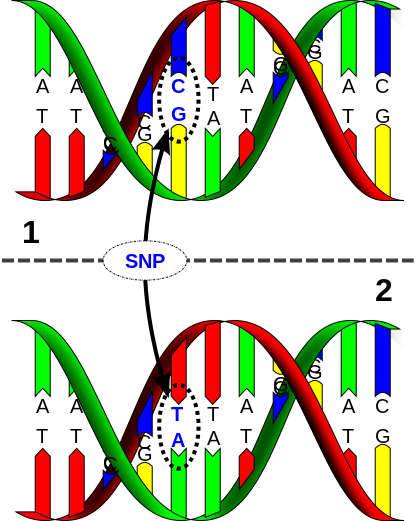
\includegraphics[scale=0.4]{SNP.png} \\
\begin{tiny}Source: http://en.wikipedia.org/wiki/File:Dna-SNP.svg\end{tiny}
\end{center}
\end{frame}

\begin{frame}{How to analyse SNPs?}
\begin{center}
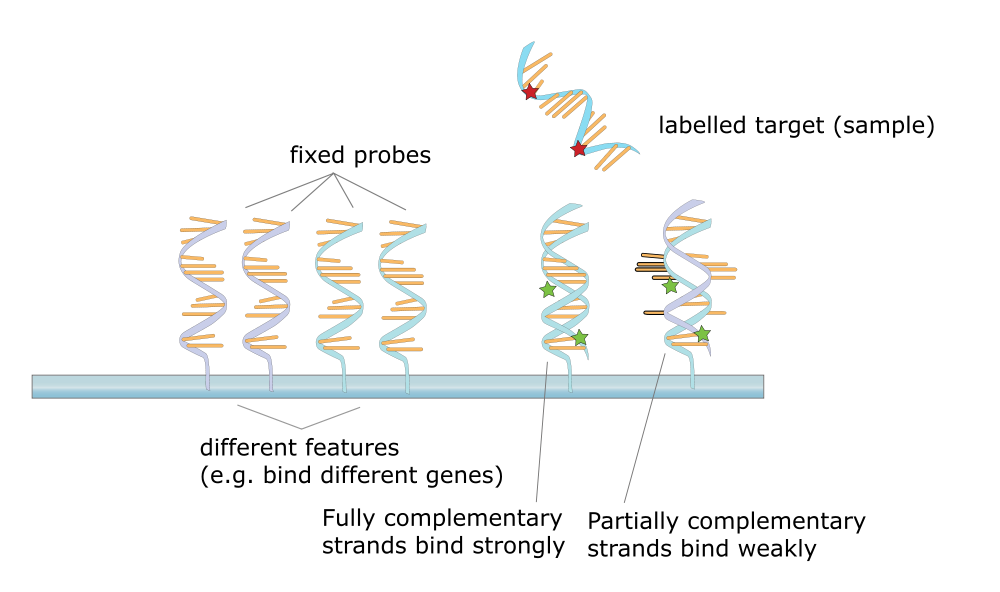
\includegraphics[scale=0.3]{microarray.png} \\
\begin{tiny}
Source: http://en.wikipedia.org/wiki/File:NA\_hybrid.svg
\end{tiny}
\end{center}
\end{frame}

\begin{frame}{How do GWAS work?}
\begin{center}
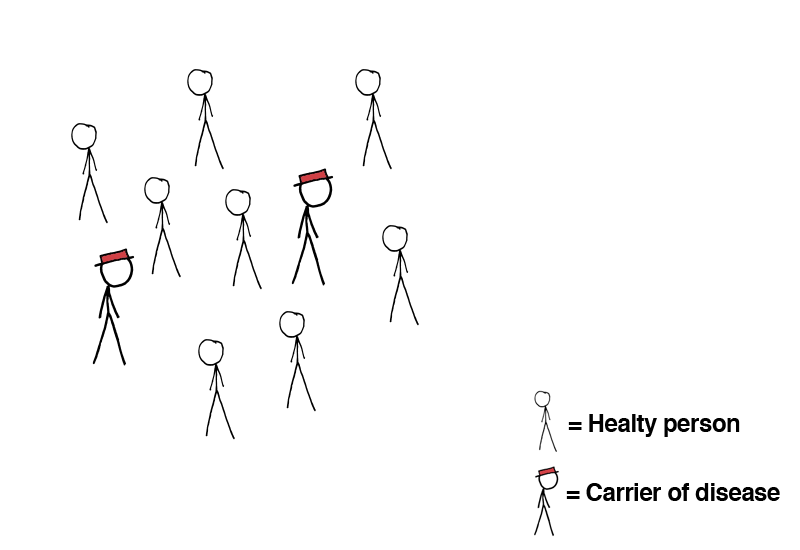
\includegraphics[scale=0.3]{distribution-disease.png} \\
\end{center}
\end{frame}

\begin{frame}{How do GWAS work?}
\begin{center}
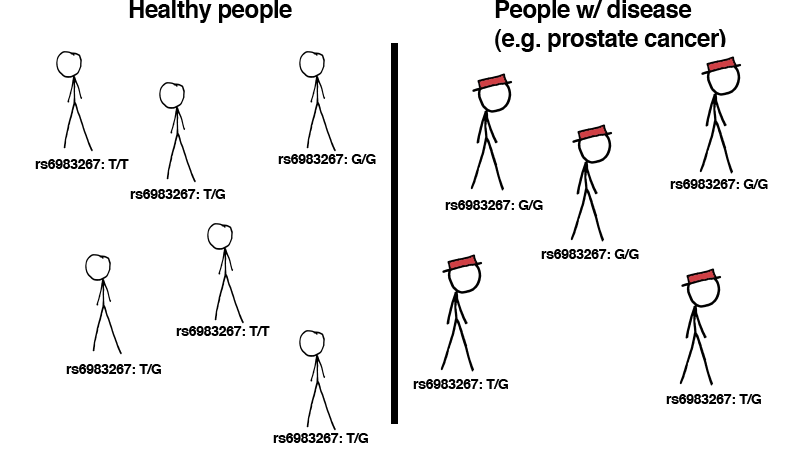
\includegraphics[scale=0.4]{gwas1.png} \\
\end{center}
\end{frame}

\begin{frame}{How do GWAS work?}
\begin{center}
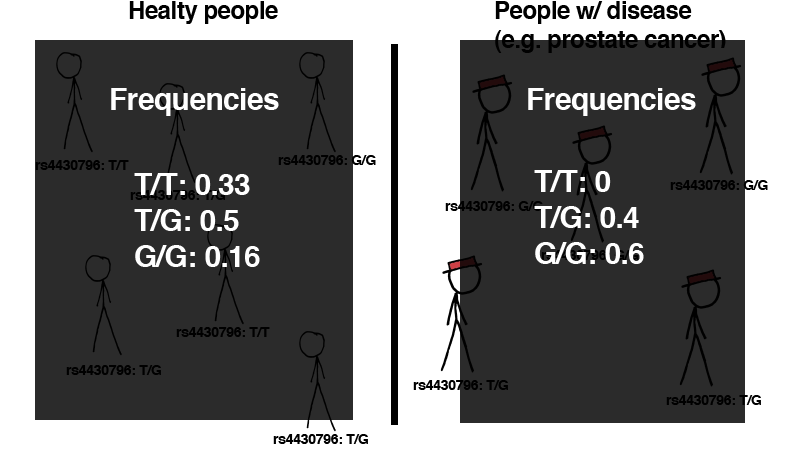
\includegraphics[scale=0.4]{gwas2.png} \\
\end{center}
\end{frame}

\begin{frame}{How do GWAS work?}
\begin{center}
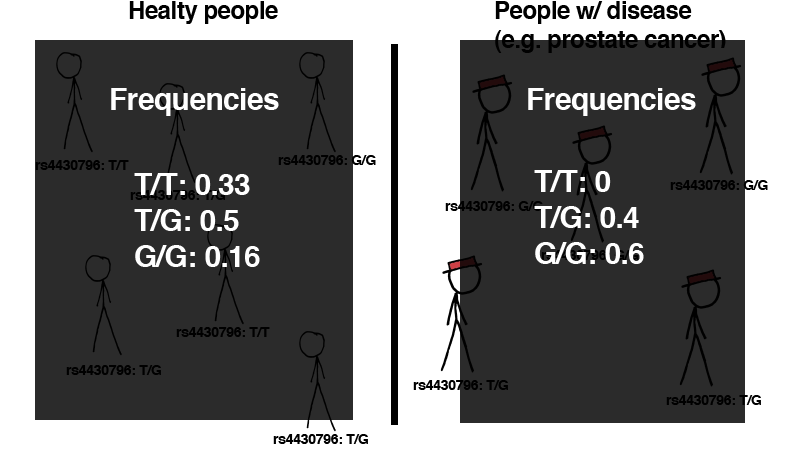
\includegraphics[scale=0.4]{gwas3.png} \\
\end{center}
\end{frame}

\begin{frame}{Some GWAS-examples}
\begin{itemize}
\item Sladek \textit{et al.} (2007) identified four gene locations linked to heightened type 2 diabetes risk
\pause \item Kogan \textit{et al.} (2011) linked rs53576 (G:G) to pro-social behaviour
\pause \item The Wellcome Trust Case Control Consortium (2007) linked 24 locations to 7 major diseases 
\end{itemize}
\end{frame}

\begin{frame}{Problems with GWAS}
\begin{flushright}

\includegraphics[scale=0.5]{doctor_xkcd.png} \\
\end{flushright}
\begin{itemize}
\item Large enough sample size
\pause \item Correcting for multiple testing
\pause \item Correlation != Causation
\end{itemize}
\end{frame}

\begin{frame}{Putting GWAS to use}
\begin{itemize}
\item Direct-To-Consumer genetic testing
\item Analyse about 1 million SNPs and provide summary of disease risks \& ancestry
\item About \$200 for a genotyping
\pause \item Providers: 23andMe, deCODEme, FamilyTree DNA, ...
\pause \item You get access to the raw data!
\end{itemize}
\begin{flushright}
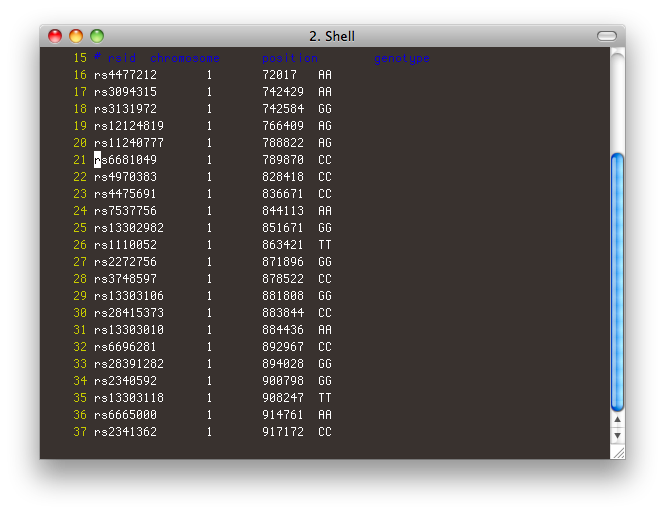
\includegraphics[scale=0.2]{23andme.png}
\end{flushright}
\end{frame}

\section{Open GWAS}
\subsection{In company vaults}

\begin{frame}{Numbers on DTC}
\begin{itemize}
\item 23andMe alone has over 100.000 customers
\pause \item 76 \% of their customers agree to participate in research
\pause \item 59 \% of them share phenotypic information with 23andMe
\end{itemize}
\end{frame}

\begin{frame}{Research in company labs}
\begin{itemize}
\item 23andMe published results of studies with up to 30.000 participants
\pause \item Replication of older GWAS
\pause \item Finding new associations for Parkinsons disease
\end{itemize}
\end{frame}

\subsection{Out of vaults}

\begin{frame}{Data sharing}
\begin{itemize}
\item People are already sharing the raw data of DTC tests 
\pause \item 1-5 \% of 23andMe customers would be enough to perform simple GWAS
\pause \item The \textit{Personal Genome Project}: Open data, but closed participation 
\end{itemize}
\end{frame}

\begin{frame}{Willing to share?}
\begin{center}
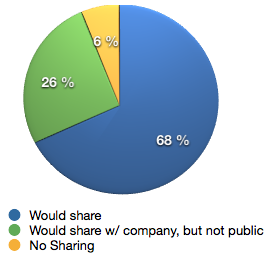
\includegraphics[scale=0.5]{pie-sharing.png}
\end{center}
\end{frame}

\begin{frame}{Willing to share?}
\begin{center}
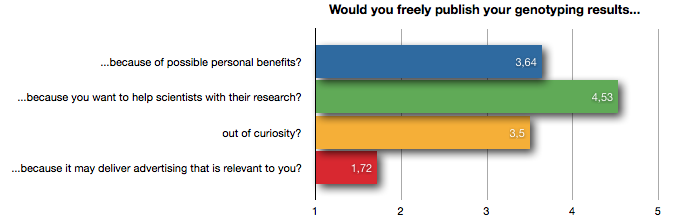
\includegraphics[scale=0.45]{sharing-reasons.png}
\end{center}
\end{frame}

\section{Privacy \& Implications}
\subsection{Some Implications}
\begin{frame}{What can happen to your open data?}
\begin{itemize}
\item Positive and negative consequences
\begin{itemize}
\pause \item Possibly extremely bad consequences
\end{itemize}
\pause \item Up to you to decide whether you want to open your data
\end{itemize}
\end{frame}

\subsection{Consequences}
\begin{frame}{Positive consequences}
\begin{itemize}
\item More knowledge about yourself
\pause \item Cheap, open science
\pause \item Great data-source for citizen scientists
\end{itemize}
\end{frame}

\begin{frame}{Negative consequences}
\begin{itemize}
\item People know more about you than you might like
\begin{itemize}
\pause \item Including your boss, insurance company, government...
\end{itemize}
%\pause \item You could be carrying a deadly disease <- Does not fit, this is a general problem of DTC tests. "Do I want to know? this does not change by making your results public
\pause \item Knowledge isn't static: Future research could show new, negative (or positive) associations. 
\pause \item Personal SNPs very similar to parents and relatives
\end{itemize}
\end{frame}

\begin{frame}{Somebody Else's Problem? A case study}
\begin{center}
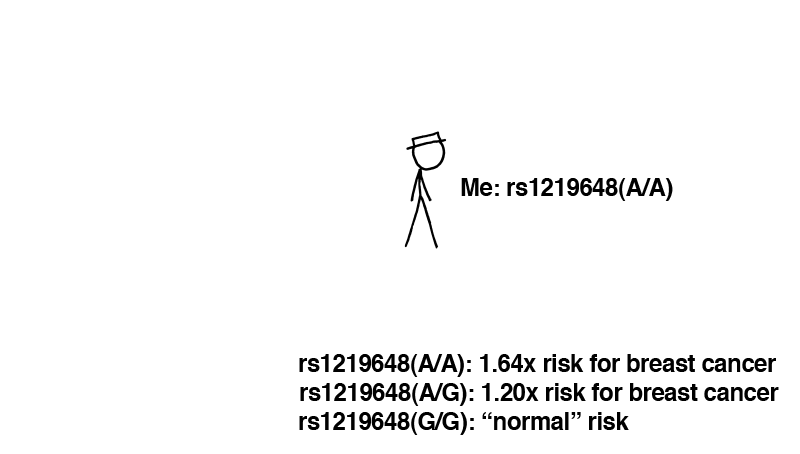
\includegraphics[scale=0.4]{privacy1.png} \\
\end{center}
\end{frame}

\begin{frame}{Somebody Else's Problem? A case study}
\begin{center}
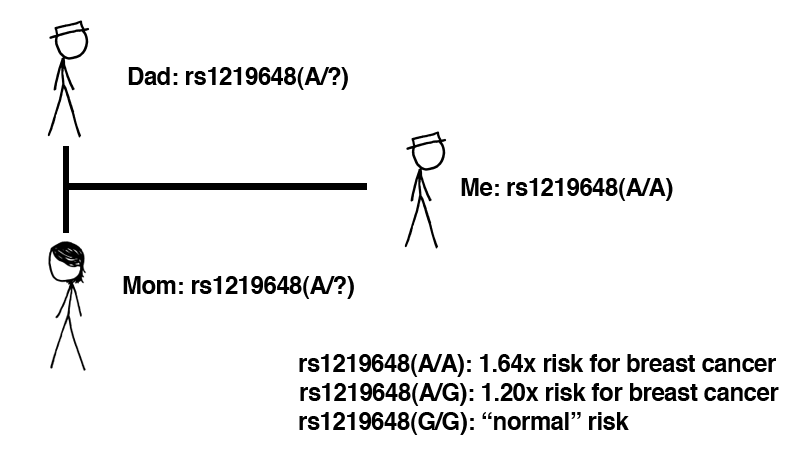
\includegraphics[scale=0.4]{privacy2.png} \\
\end{center}
\end{frame}

\begin{frame}{Somebody Else's Problem? A case study}
\begin{center}
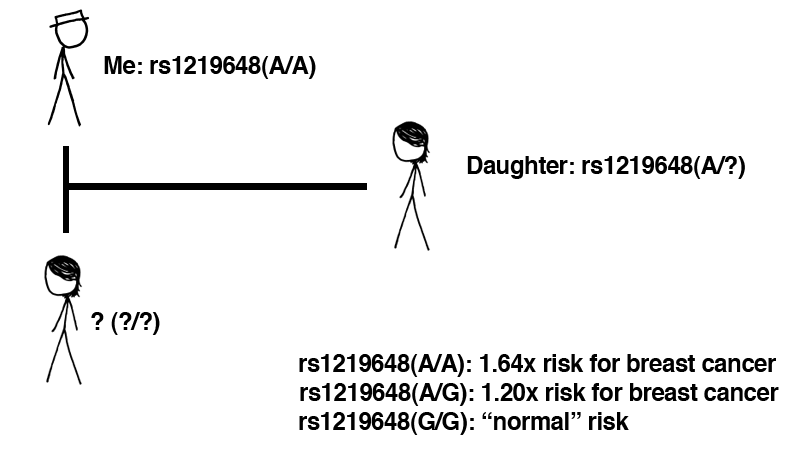
\includegraphics[scale=0.4]{privacy3.png} \\
\end{center}
\end{frame}

% maybe put this under positive consequences? 
\begin{frame}{Possible Solutions}
\begin{itemize}
\item What about laws?
\begin{itemize} 
\pause \item US: Genetic Information Nondiscrimination Act (GINA, 2008)
\pause \item Germany: Gendiagnostikgesetz (GenDG, 2010)
\end{itemize}
\end{itemize}
\end{frame}

\begin{frame}{Open GWAS}
\begin{itemize}
\item No central repository for open genotypings!
\pause \item We've created openSNP.org
\pause \item open source repository for CC0-genotypings from 23andme, deCODEme and others
\pause \item Allows users to annotate with phenotypes (hair colour, nicotine dependence...)
\pause \item Everybody can download everything
\pause \item So far: 78 genotypings and 188 users % change before talk
\end{itemize}
\end{frame}

\section{Discussion}
% slight repition
\begin{frame}{Conclusions}
\begin{itemize}
\item Open GWAS are the future of personalised medicine
\pause \item It's in the hands of users to make or break the situation
\pause \item Chance to take science into our own hands %meh
\end{itemize}
\end{frame}

\subsection{Outlook}
\begin{frame}{Future of openSNP}
\begin{itemize}
\item We've won the PLoS/Mendeley Binary Battle
\pause \item Constantly improving the project
\pause \item Trying to get funds for free genotypings
\end{itemize}
\end{frame}

\begin{frame}{The end}
\begin{center}
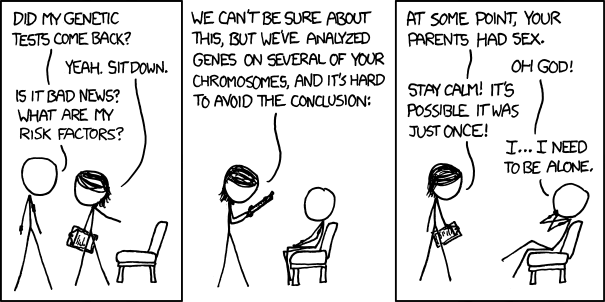
\includegraphics[scale=0.5]{genetic_analysis.png} \\
Thanks for listening. Any questions?
\end{center}
\end{frame}


\begin{frame}{References}
\begin{tiny}
Kogan, \textit{et al.} (2011): Thin-slicing study of the oxytocin receptor (OXTR) gene and the evaluation and expression of the prosocial disposition. Proceedings of the National Academy of Sciences\\
Sladek \textit{et al.} (2007): "A genome-wide association study identifies novel risk loci for type 2 diabetes". Nature 445 (7130): 881-5. \\
The Wellcome Trust Case Control Consortium  (2007): Genome-wide association study of 14,000 cases of seven common diseases and 3,000 shared controls. Nature 447: 661-678.\\
\end{tiny}
\end{frame}
\end{document}
